\documentclass[11pt]{article}
\usepackage[margin=1in]{geometry}
\usepackage{graphicx}
\usepackage{booktabs}
\usepackage{amsmath}
\usepackage{hyperref}

\title{Quantum Support Vector Machines for Sample-Efficient Haemorrhagic Fever Strain Differentiation}
\author{}
\date{}

\begin{document}
\maketitle

\begin{abstract}
Clinical differentiation of Bundibugyo, Zaire, Sudan, and non-Ebola haemorrhagic fever is difficult during early outbreak response, particularly when molecular testing is delayed or calibrated for the wrong strain. We evaluate a Quantum Support Vector Machine (QSVM) with a ZZFeatureMap-inspired kernel for rare-class recall in an imbalanced triage setting. Patient-level records are reconstructed from published clinical frequency tables using individual patient data reconstruction from summary statistics. Classical baselines include linear SVM, RBF SVM, random forest, logistic regression, and XGBoost. The primary endpoint is Bundibugyo recall, with macro recall, ROC-AUC, average precision, McNemar tests, learning curves, and geometric difference used as secondary analyses. This scaffold should be completed with measured values from \texttt{results/metrics/} after the full pipeline is run.
\end{abstract}

\section{Introduction}
The 2026 Bundibugyo Ebola emergency highlights a practical diagnostic problem: strain-specific test availability can lag clinical suspicion. A bedside triage classifier cannot replace PCR confirmation, but it may help prioritise isolation and urgent sampling where laboratory capacity is limited.

\section{Background}
Quantum support vector machines use a feature map $U(x)$ to embed classical observations into a Hilbert space. The kernel is
\[
K(x_i, x_j) = |\langle 0 | U^\dagger(x_j) U(x_i) | 0 \rangle|^2.
\]
The implemented feature map uses Hadamard gates, angle encoding, and neighbouring ZZ interactions to represent pairwise symptom co-occurrence.

\section{Data and Features}
Data are reconstructed from summary statistics in peer-reviewed sources: MacNeil et al. 2010, doi:10.3201/eid1612.100627; Roddy et al. 2012, doi:10.1371/journal.pone.0052986; Kiggundu et al. 2022, doi:10.15585/mmwr.mm7145a5; Schieffelin et al. 2014, doi:10.1056/NEJMoa1411680. WHO Situation Report 01, dated 18 May 2026, is used for outbreak context.

The feature set contains 20 binary symptoms and derived clinical severity scores. HDX CSV files are aggregate epidemiological context only and are not used as patient-level clinical features.

\section{Methodology}
Records are reconstructed by Bernoulli sampling each symptom from its source-cohort frequency with random seed 42. Features are standardised, reduced to six principal components, and scaled to $[0,\pi]$ for quantum encoding. Train/test splits are stratified; SMOTE is applied only to the training set. Classical models are fit before the QSVM.

\section{Results}
Insert final metric tables from \texttt{results/metrics/classical_results.json} and \texttt{results/metrics/qsvm_results.json}.

\begin{figure}[h]
\centering
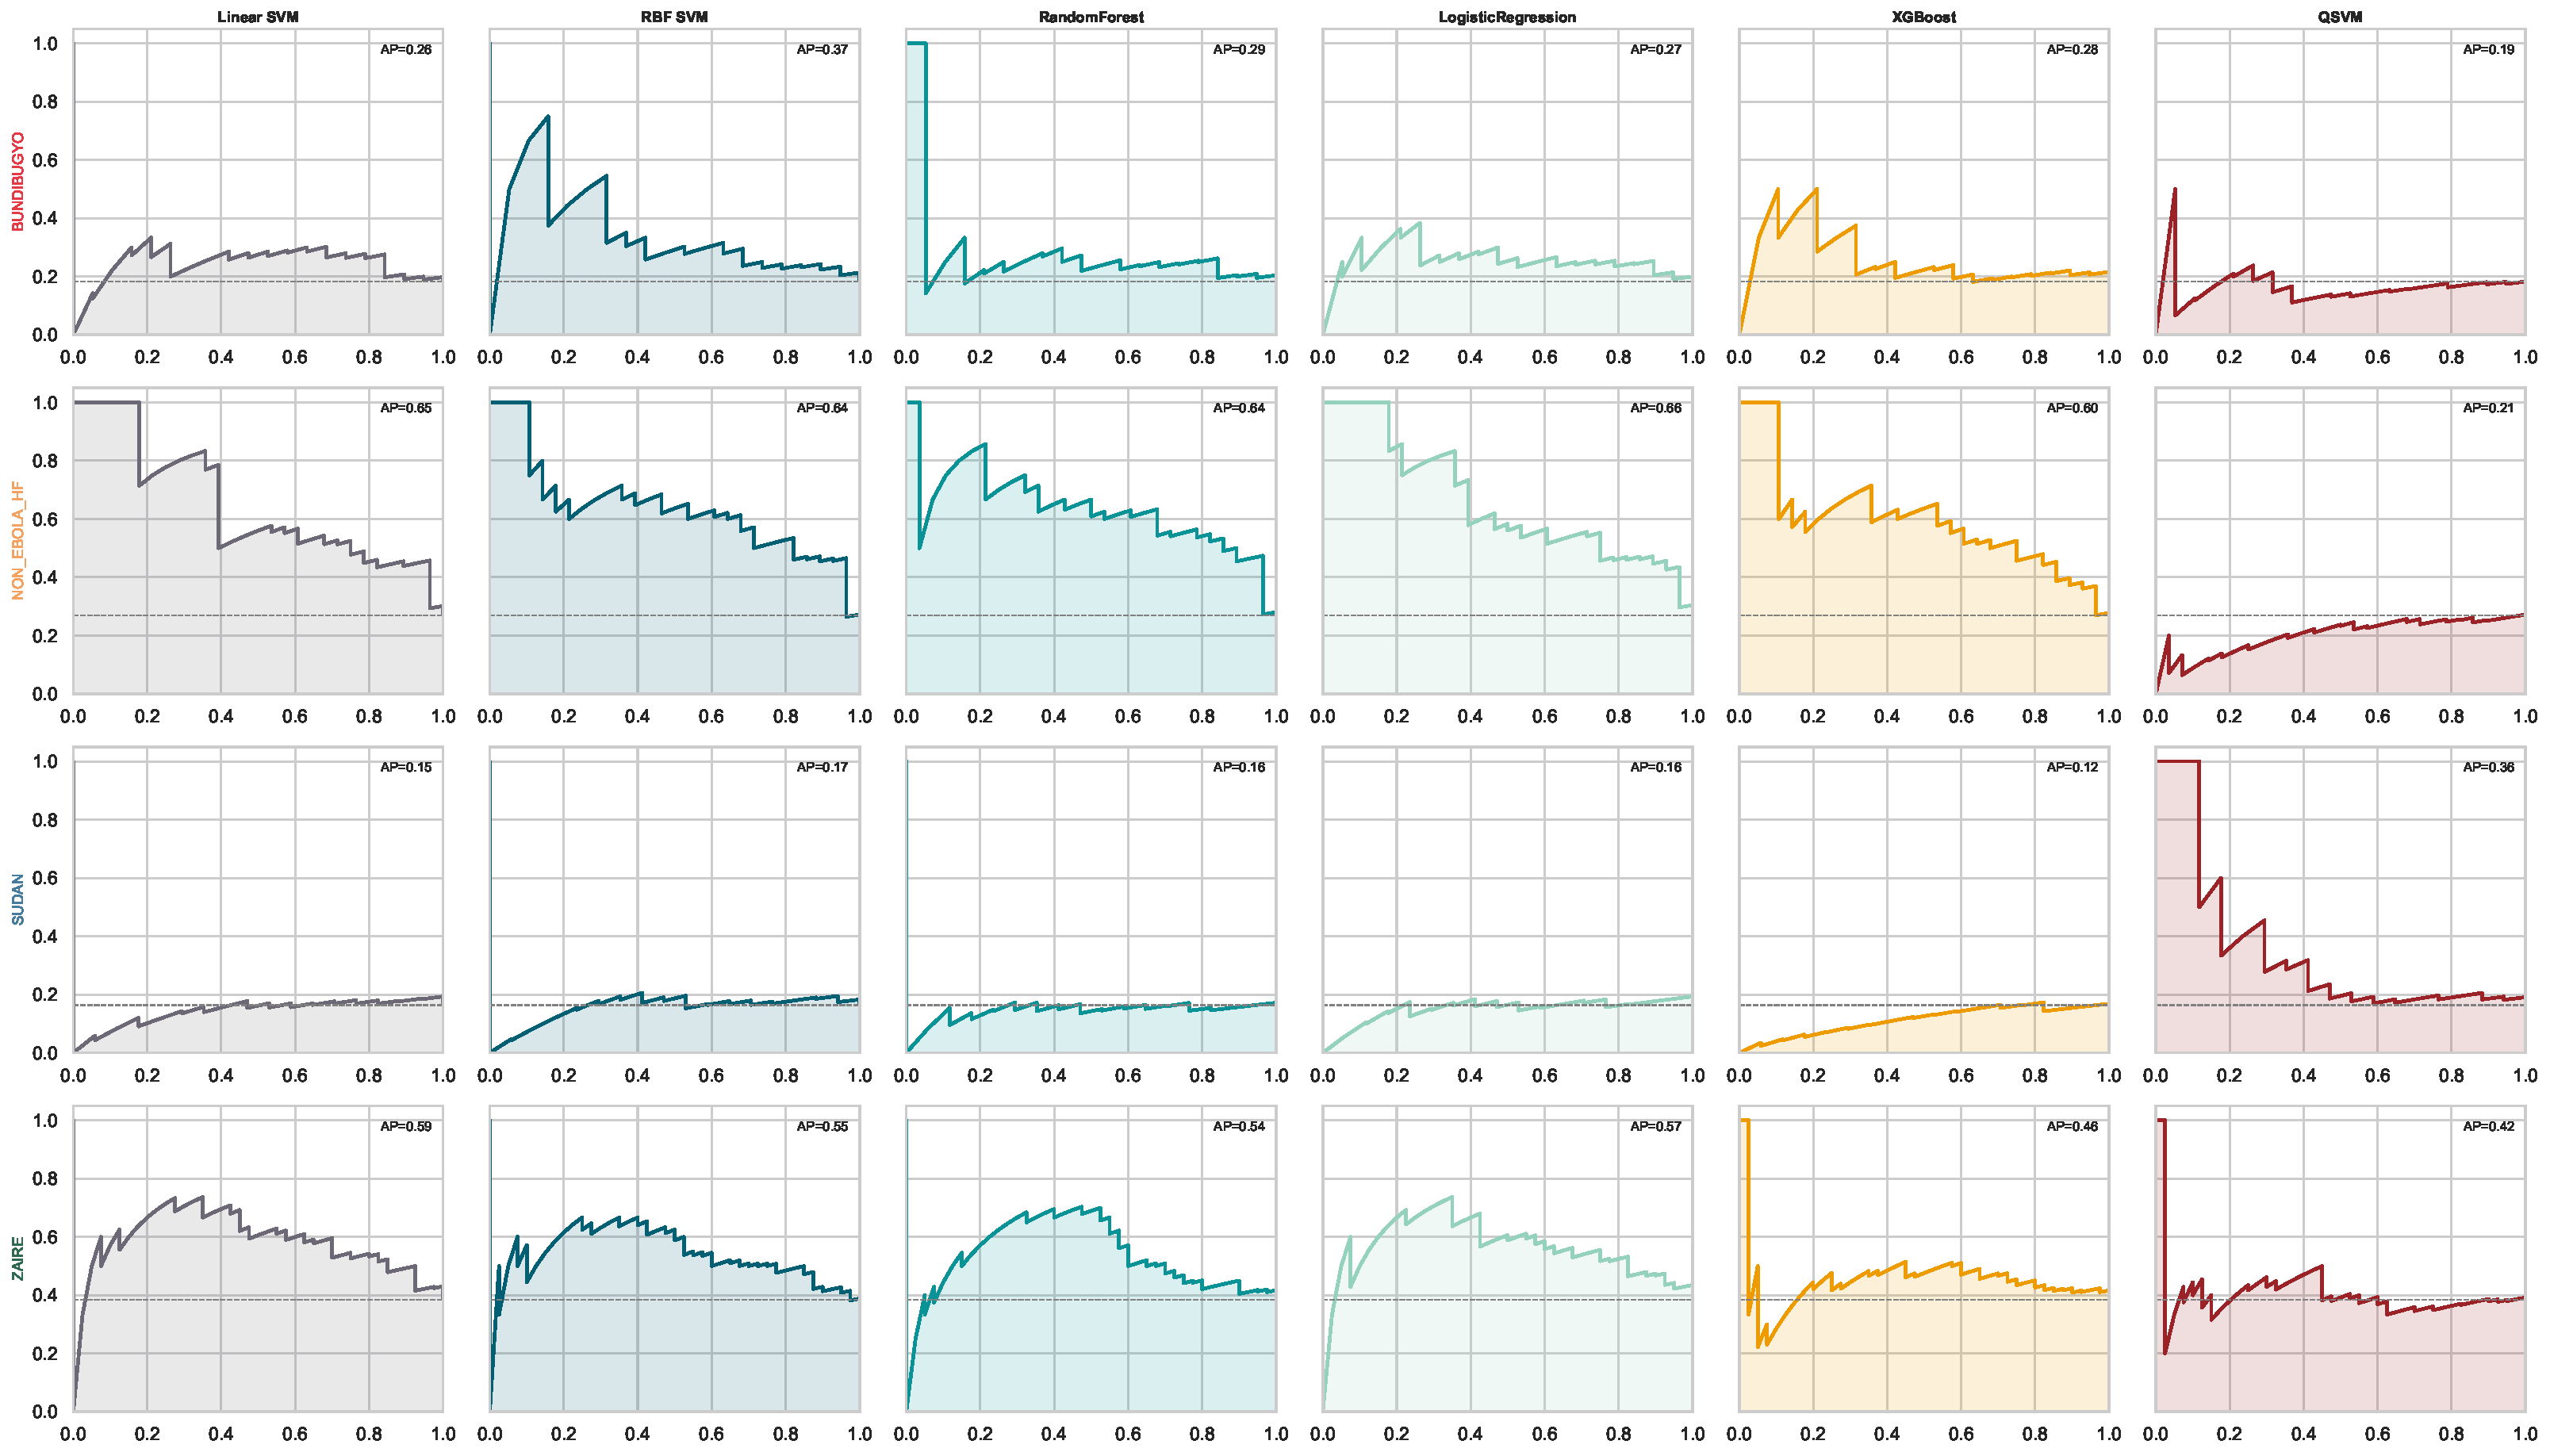
\includegraphics[width=\linewidth]{../results/figures/precision_recall_grid.pdf}
\caption{Per-class precision-recall curves.}
\end{figure}

\begin{figure}[h]
\centering
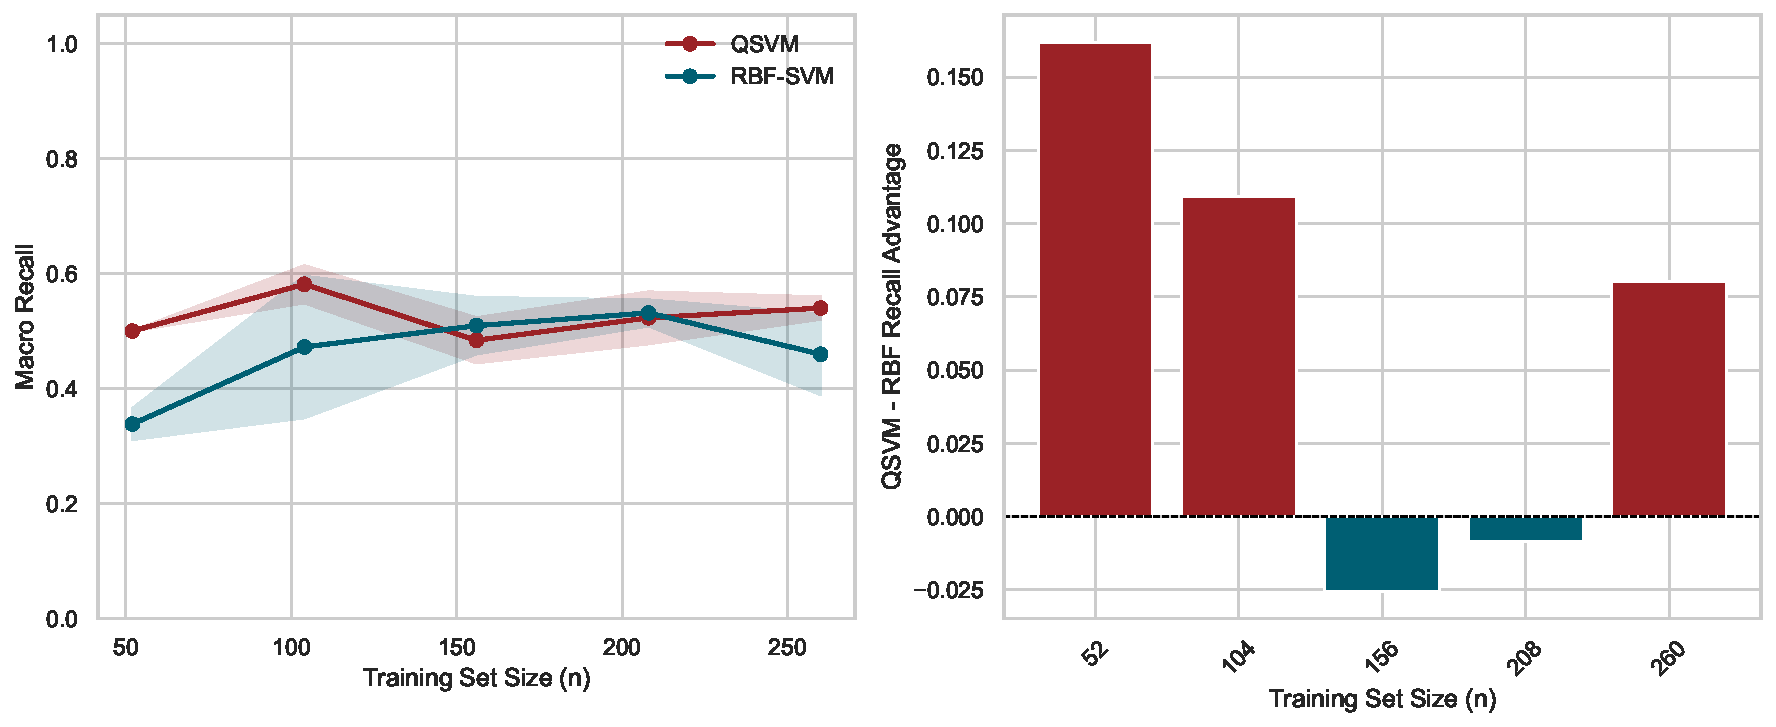
\includegraphics[width=\linewidth]{../results/figures/sample_complexity.pdf}
\caption{Sample-complexity comparison.}
\end{figure}

\begin{figure}[h]
\centering
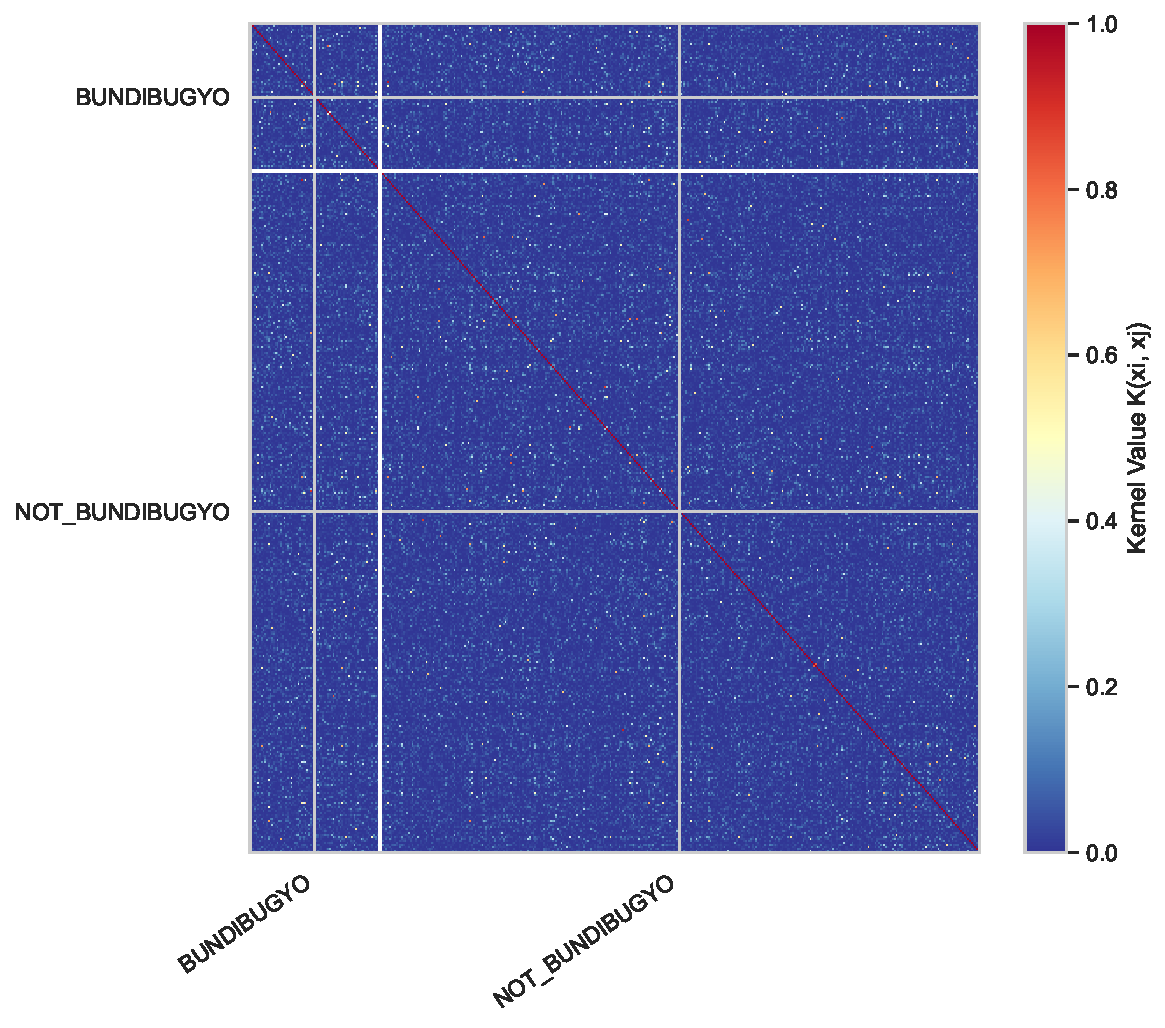
\includegraphics[width=0.8\linewidth]{../results/figures/kernel_matrix_heatmap.pdf}
\caption{Quantum kernel matrix sorted by class.}
\end{figure}

\begin{figure}[h]
\centering
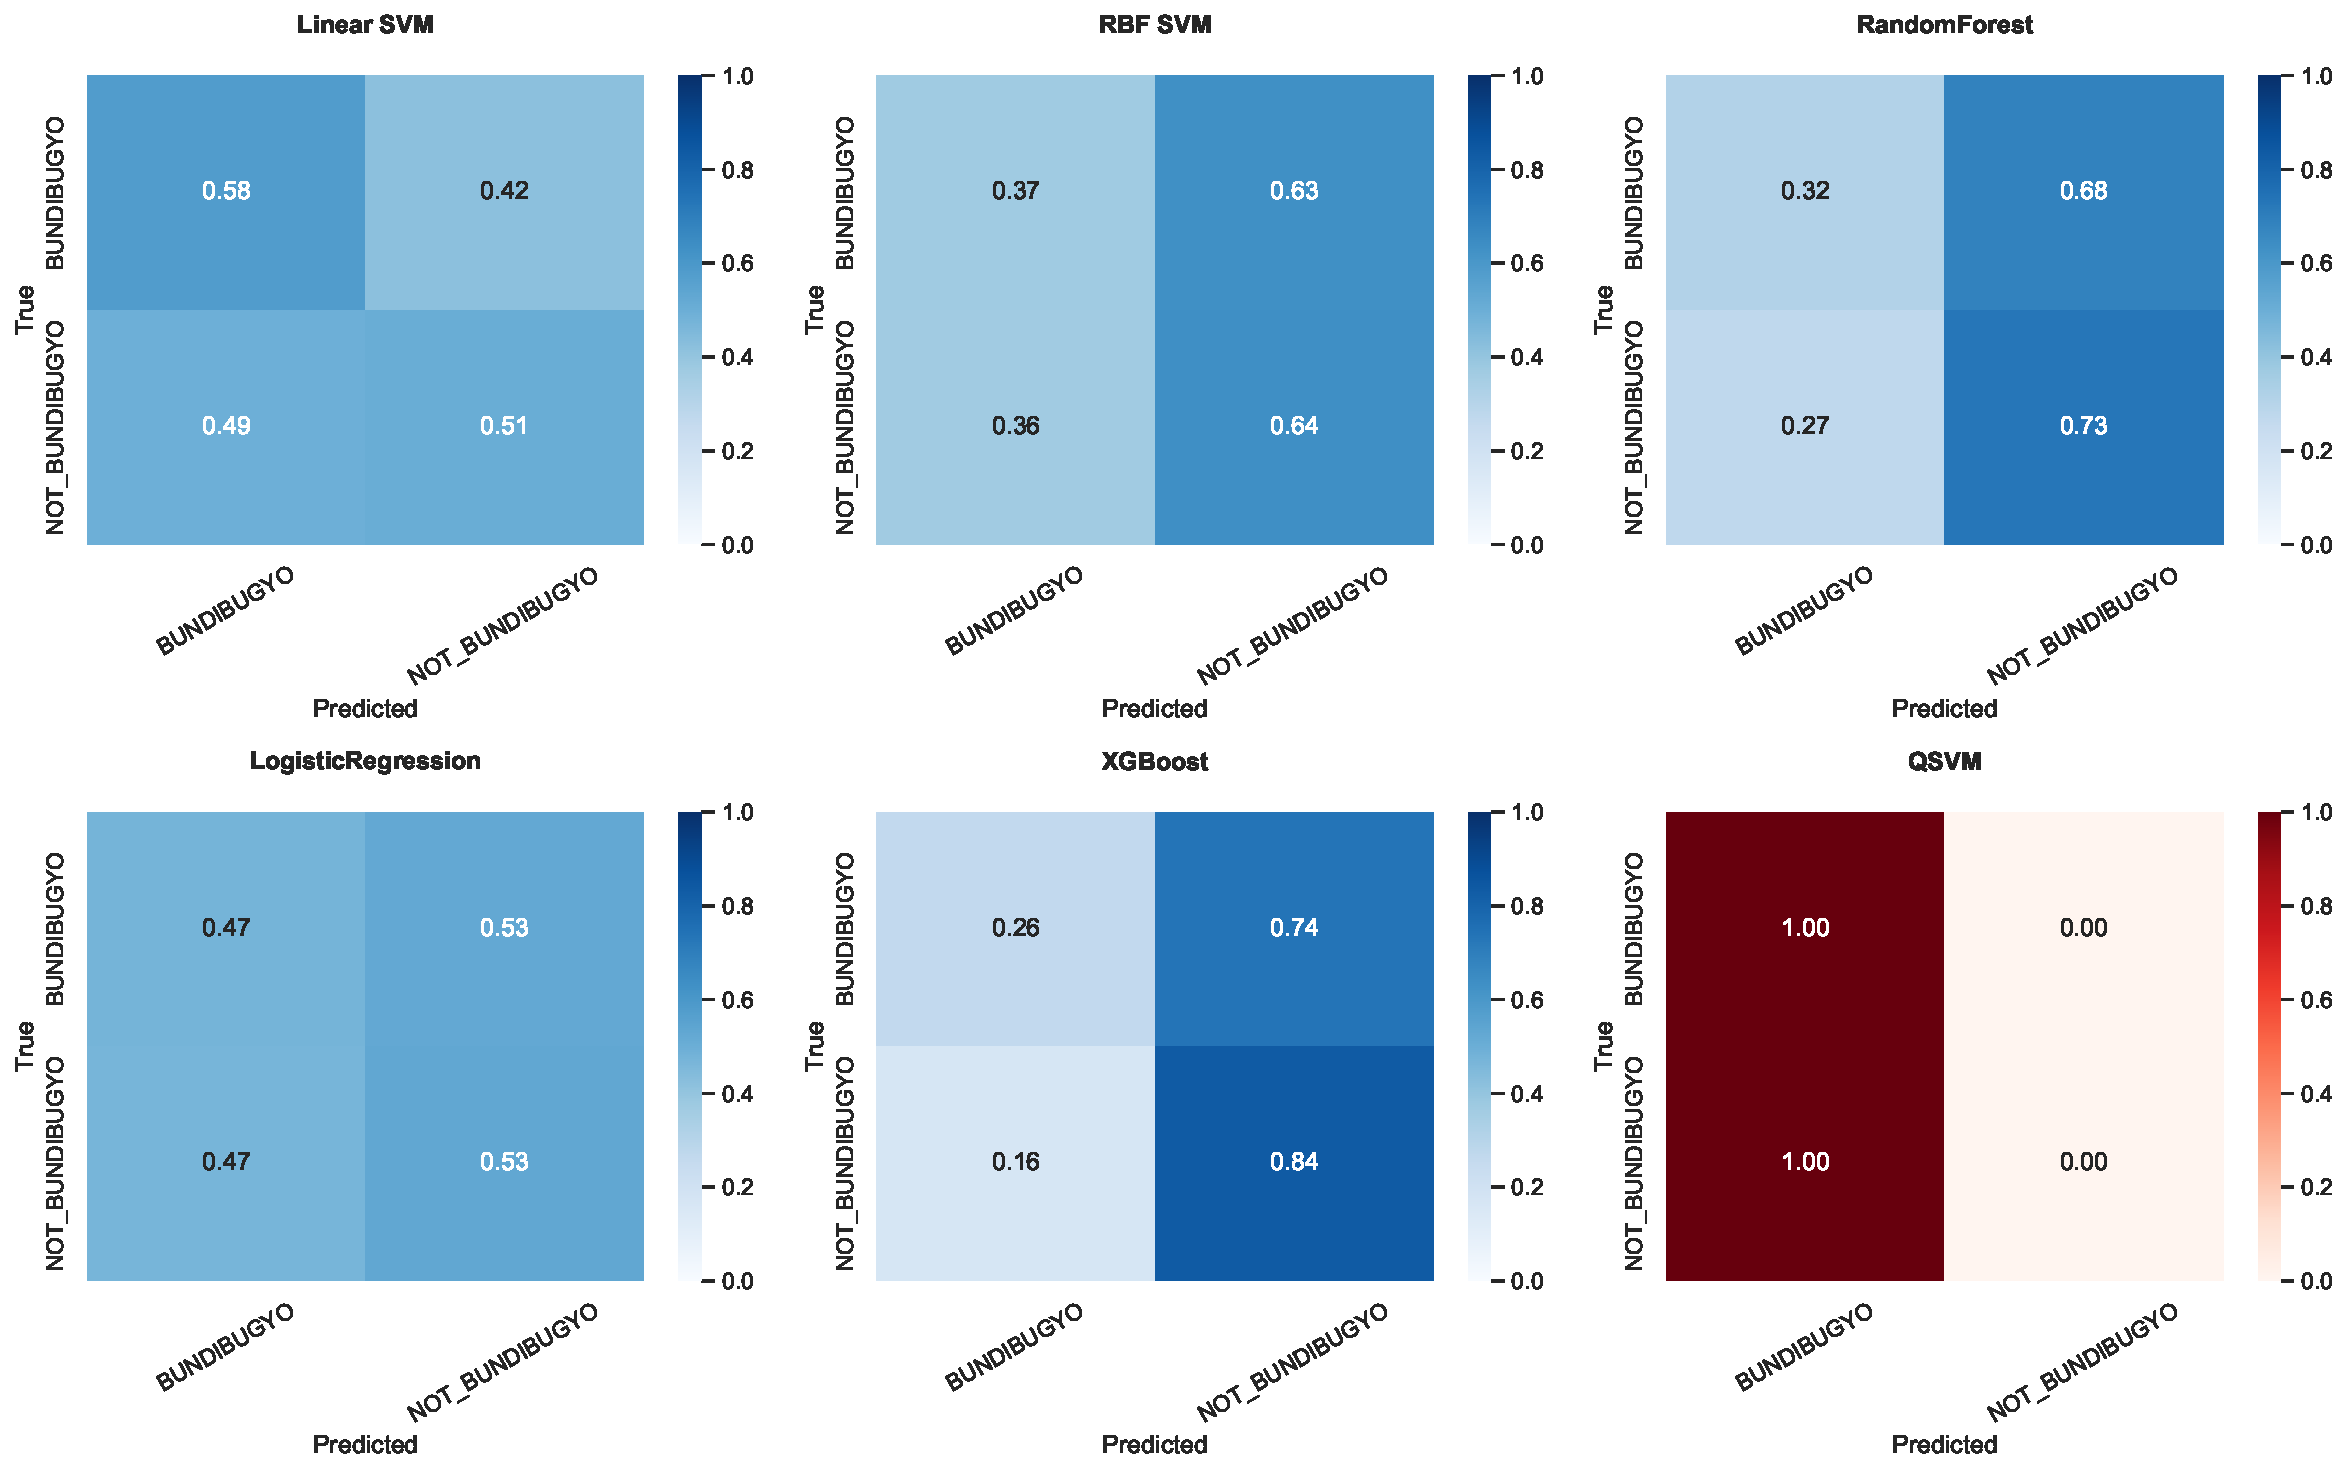
\includegraphics[width=\linewidth]{../results/figures/confusion_matrix_comparison.pdf}
\caption{Normalised confusion matrix comparison.}
\end{figure}

\section{Discussion}
The central clinical concern is recall on the rare but operationally critical Bundibugyo class. Any quantum advantage claim should be restricted to results supported by held-out recall, statistical tests, and geometric difference.

\section{Limitations}
The training set is reconstructed from published summaries rather than raw patient records. The quantum kernel is initially evaluated on a simulator. Prospective validation on clinical data is required before deployment.

\section{Conclusion}
This project provides a reproducible benchmark for QSVM-based haemorrhagic fever strain triage under class imbalance and limited data.

\section*{References}
\begin{itemize}
\item MacNeil et al. 2010. Emerging Infectious Diseases. doi:10.3201/eid1612.100627.
\item Roddy et al. 2012. PLoS ONE. doi:10.1371/journal.pone.0052986.
\item Kiggundu et al. 2022. MMWR. doi:10.15585/mmwr.mm7145a5.
\item Schieffelin et al. 2014. New England Journal of Medicine. doi:10.1056/NEJMoa1411680.
\item WHO Situation Report 01, 18 May 2026.
\end{itemize}

\end{document}
